\documentclass[12pt]{beamer}
%\documentclass[20pt,handout]{beamer}
\usetheme{Darmstadt}
\usepackage{graphicx}
\usepackage[ngerman]{babel}
\usepackage[T1]{fontenc}
\usepackage[utf8]{inputenc}
\usepackage{tikz}
\usepackage[shadow,colorinlistoftodos]{todonotes}
\setbeamertemplate{footline}[frame number]

\newcommand{\cc}[1]{\includegraphics[height=4mm]{img/#1.png}}
\usepackage{ifthen}
\newcommand{\license}[2][]{\\#2\ifthenelse{\equal{#1}{}}{}{\\\scriptsize\url{#1}}}
\usepackage{textcomp}

\setbeamercovered{transparent}

\pgfdeclareimage[height=.6cm]{c3d2logo}{./img/c3d2.pdf} 


\pgfdeclarelayer{foreground}
\pgfsetlayers{main,foreground}
\logo{\pgfputat{\pgfxy(-1,0)}{\pgfbox[center,base]{\pgfuseimage{c3d2logo}}}}


\title{Chaos macht Schule}
\author{\small Robert Wartenberg \& Benjamin Partzsch\\\large Chaos Computer Club Dresden}
\date{26.06.2018}

\begin{document}
\maketitle

\section{Einleitung}
\subsection{}

%%% -> J03 -> %%%

\begin{frame}
  \frametitle{Hacker}
  \begin{figure}
    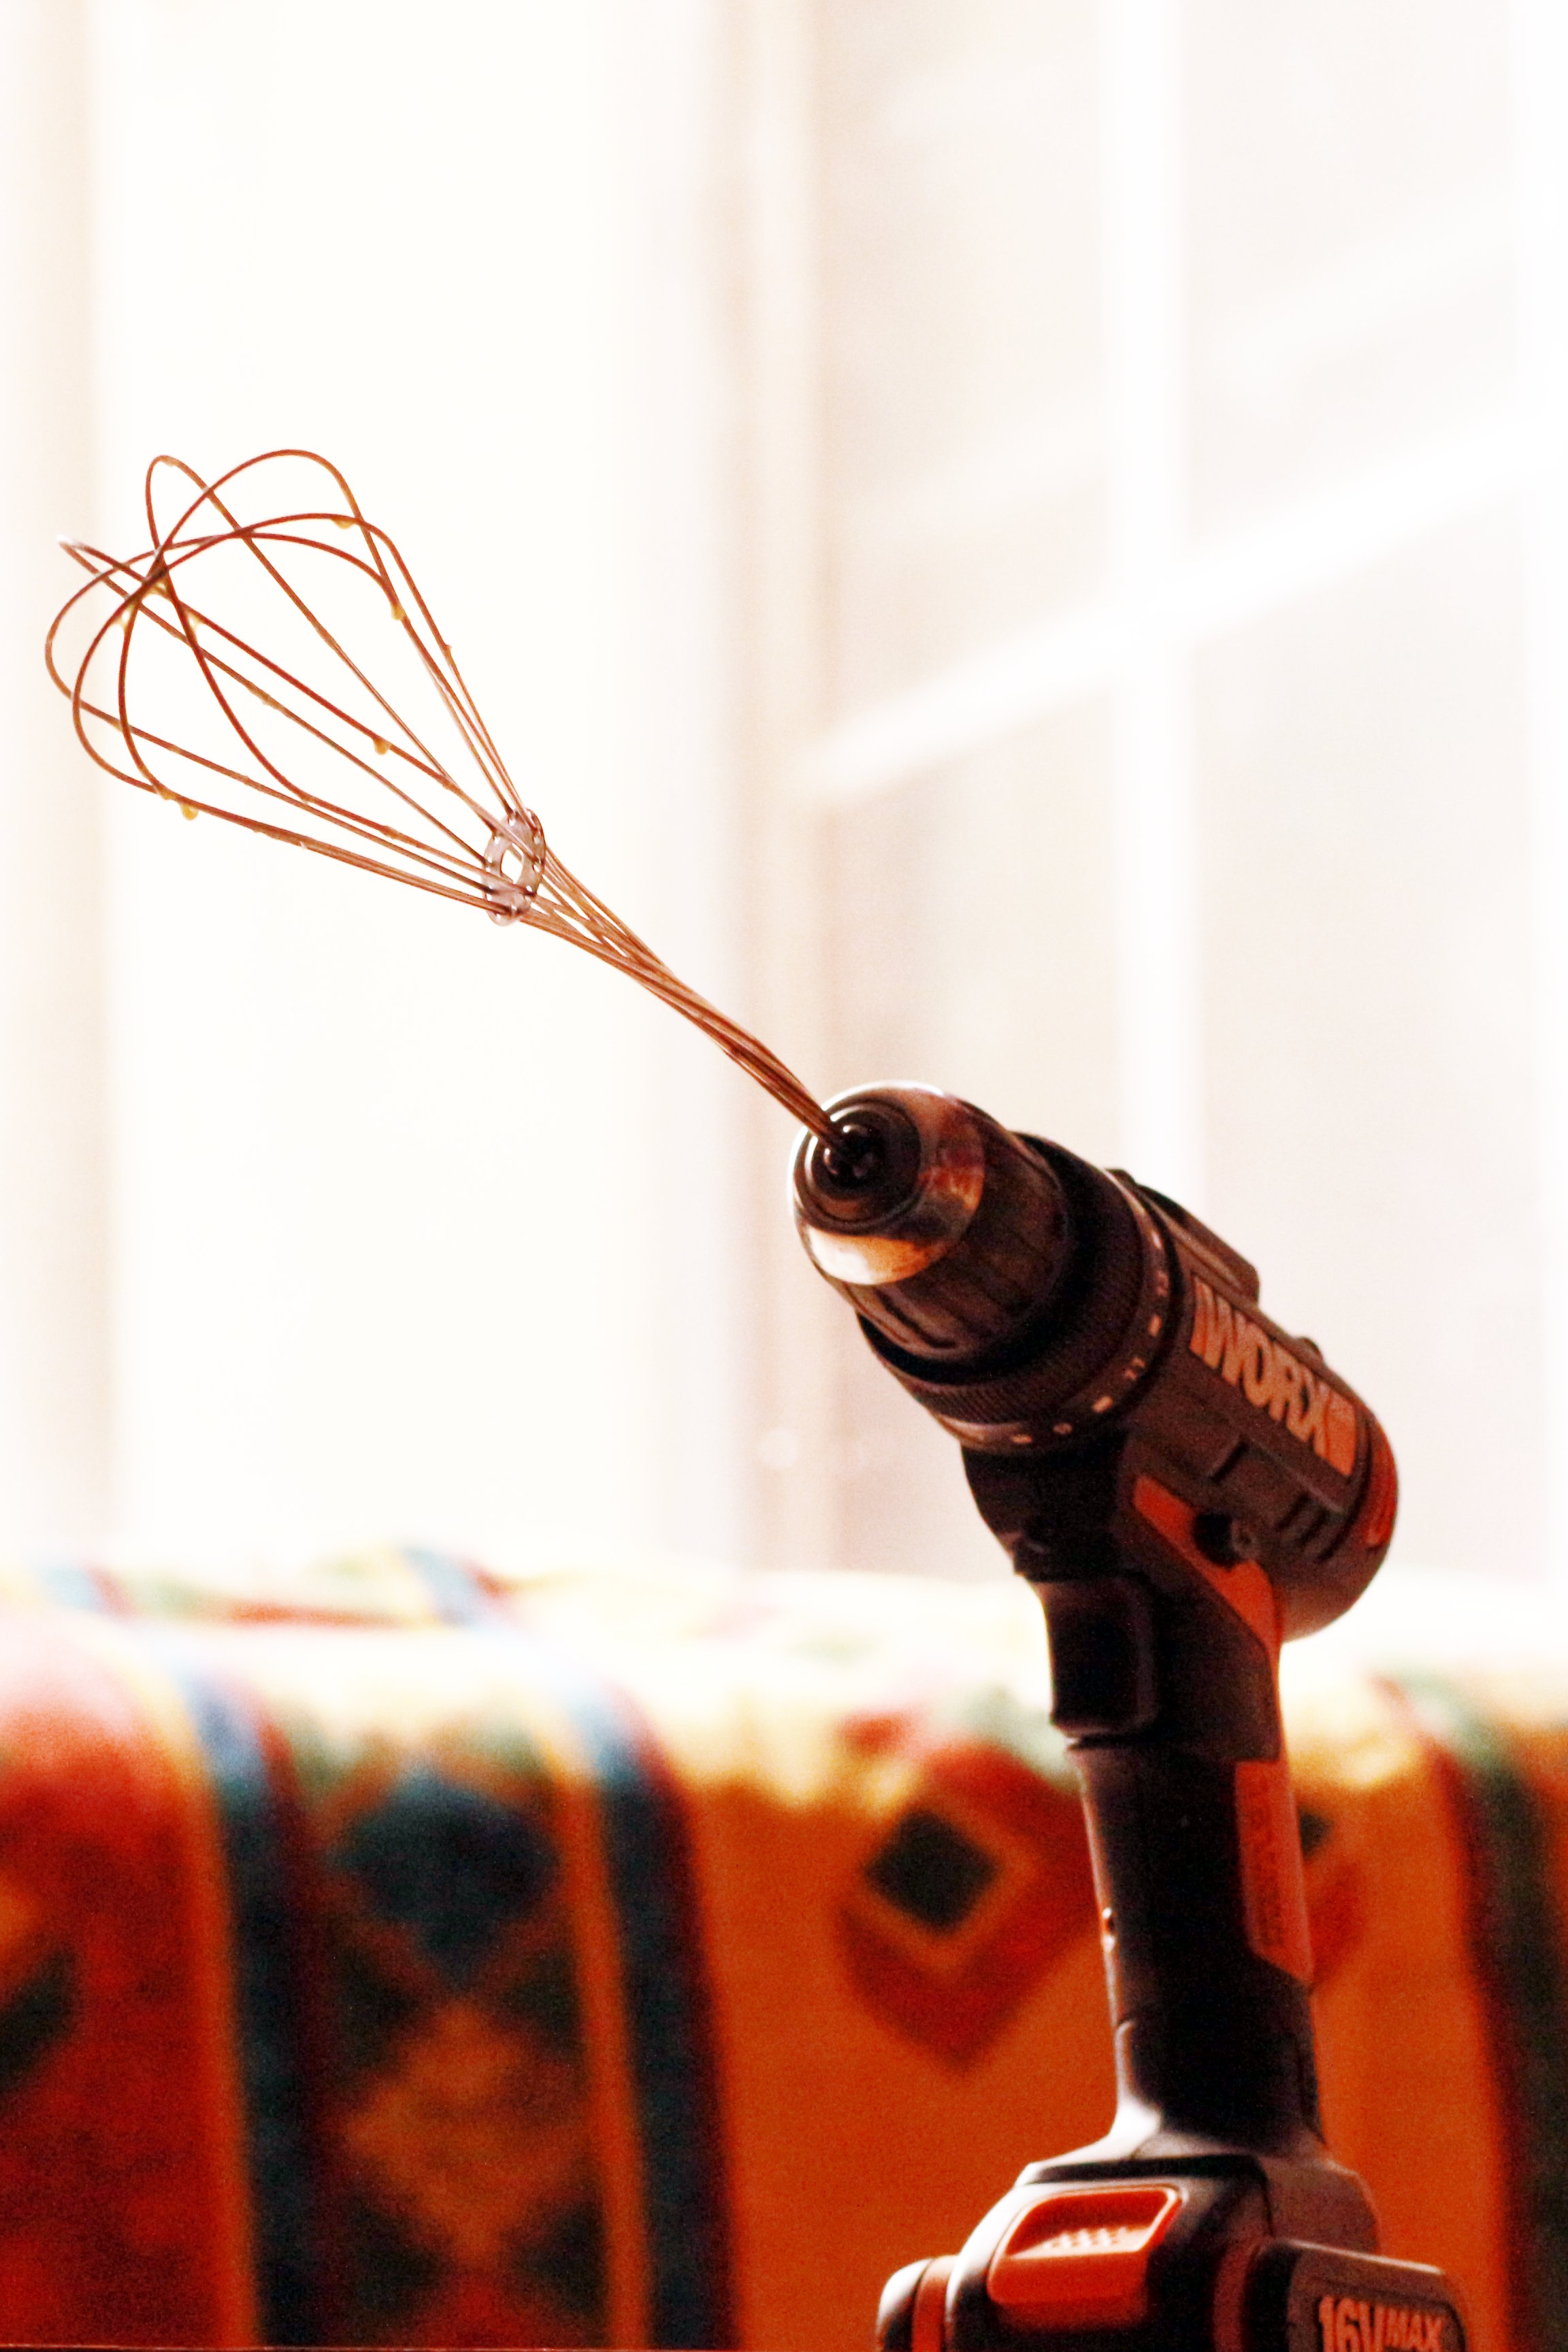
\includegraphics[height=0.7\textheight]{img/schneeschrauber.jpg}
  \end{figure}
\end{frame}

\begin{frame}
	\begin{center}
    	
\includegraphics[height=0.5\textheight]{img/cms-text.png}
    \end{center}
\end{frame}

\begin{frame}
	\frametitle{Chaos Computer Club}
	\begin{center}
		
\includegraphics[height=0.2\textheight]{img/chaosknoten.png}
	\end{center}	
	\begin{itemize}
		\item Verein wurde 1981 gegründet (\url{https://ccc.de})          
		\item Aktuell mehr als 6000 Mitglieder
		\item Betreibt u.a. Öffentlichkeitsarbeit und Politikberatung      
		\item Lokale Erfahrungsaustauschkreise (Erfas) und Chaostreffs
	\end{itemize}
\end{frame}

\begin{frame}
	\frametitle{Chaos Computer Club Dresden}
	\begin{center}
		
\includegraphics[height=0.1\textheight]{img/c3d2_logo.png}
	\end{center}
	\begin{itemize}
		\item Chaos Computer Club Dresden (\url{https://c3d2.de})          
		\item Datenspuren (\url{https://datenspuren.de})
		\item Radio und Podcasts (\url{https://c3d2.de/radio.html})
		\item Chaos macht Schule (\url{https://c3d2.de/schule.html})
	\end{itemize}
\end{frame}
  
%%% -> Rob -> %%%

\section{CmS}
\subsection{}

\begin{frame}
	\begin{center}
    	
\includegraphics[height=0.5\textheight]{img/cms-text.png}
    \end{center}
\end{frame}
  
\begin{frame}
	\frametitle{Chaos macht Schule}
	\begin{itemize}
		\item<1-> seit ca. 2007
		\item<2-> Ehrenamtlich organisiert
		\item<3-> Bildung und Sensibilisierung
	\end{itemize}
\end{frame}
  
\begin{frame}
	\frametitle{Zielgruppe}
	\begin{itemize}
		\item<1-> Schüler*innen
		\item<2-> Lehrer*innen
		\item<3-> Eltern 
	\end{itemize}
\end{frame}
  
%%% -> J03 -> %%%

\begin{frame}
	\frametitle{Inhalte}
	\begin{itemize}
		\item<1-> Datenschutz statt Überwachung
			\only<1>{
				\begin{center}
				
\includegraphics[height=0.7\textheight]{img/snowden.jpg}
				\end{center}
			}
			\only<2>{
				\begin{center}
				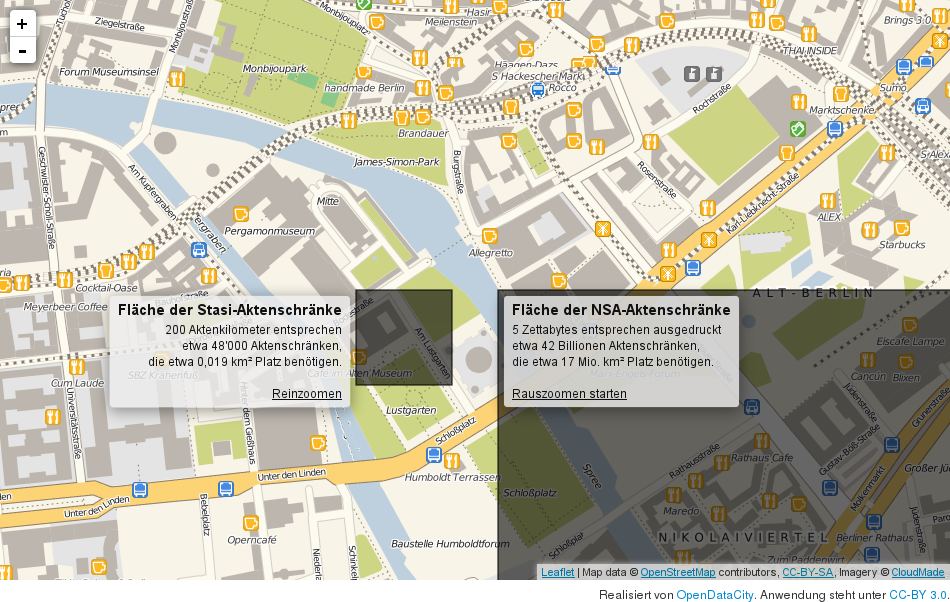
\includegraphics[height=0.7\textheight]{img/akten1.png}
				\end{center}
			}
			\only<3>{
				\begin{center}
				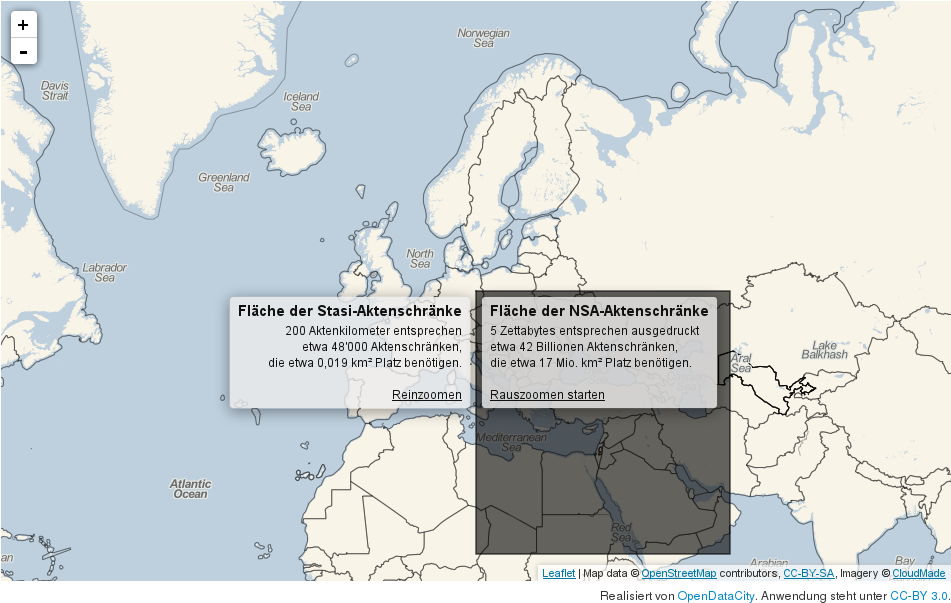
\includegraphics[height=0.7\textheight]{img/akten2.png}
				\end{center}
			}
			\only<4>{
				\begin{center}
				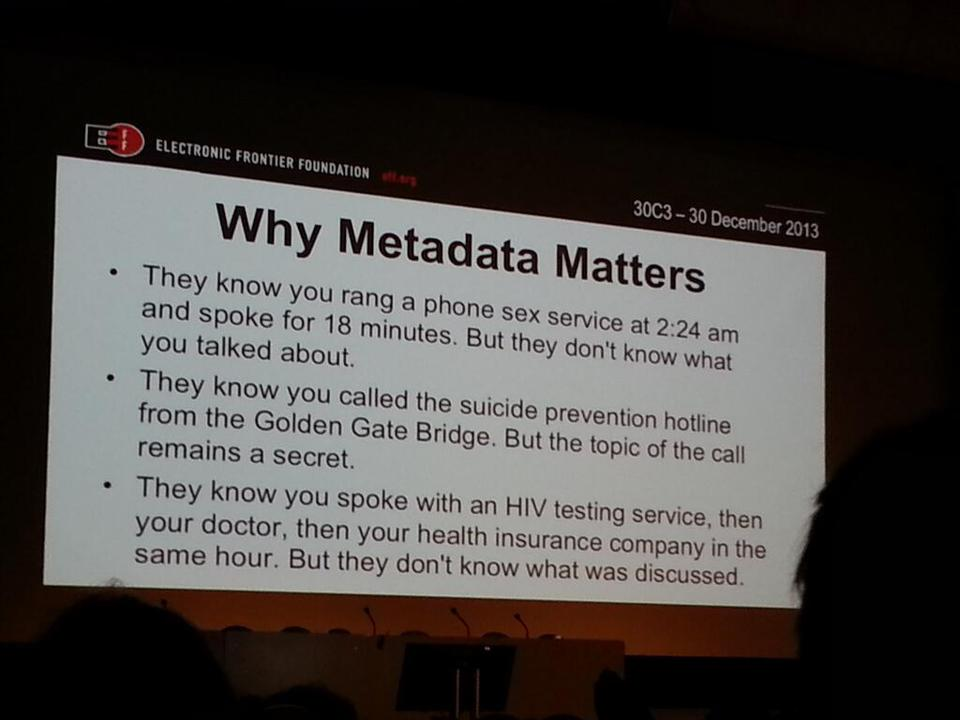
\includegraphics[height=0.7\textheight]{img/metadata-matters.jpg}
				\end{center}
			}
		\item<5-> Sensibilisierung für freie Software \& Dienste
			\only<5>{
				\begin{center}				
				
\includegraphics[height=0.7\textheight]{img/business_pigs.jpg}
				\end{center}
			}
		\item<6-> Workshops
			\only<6>{
				\begin{center}
				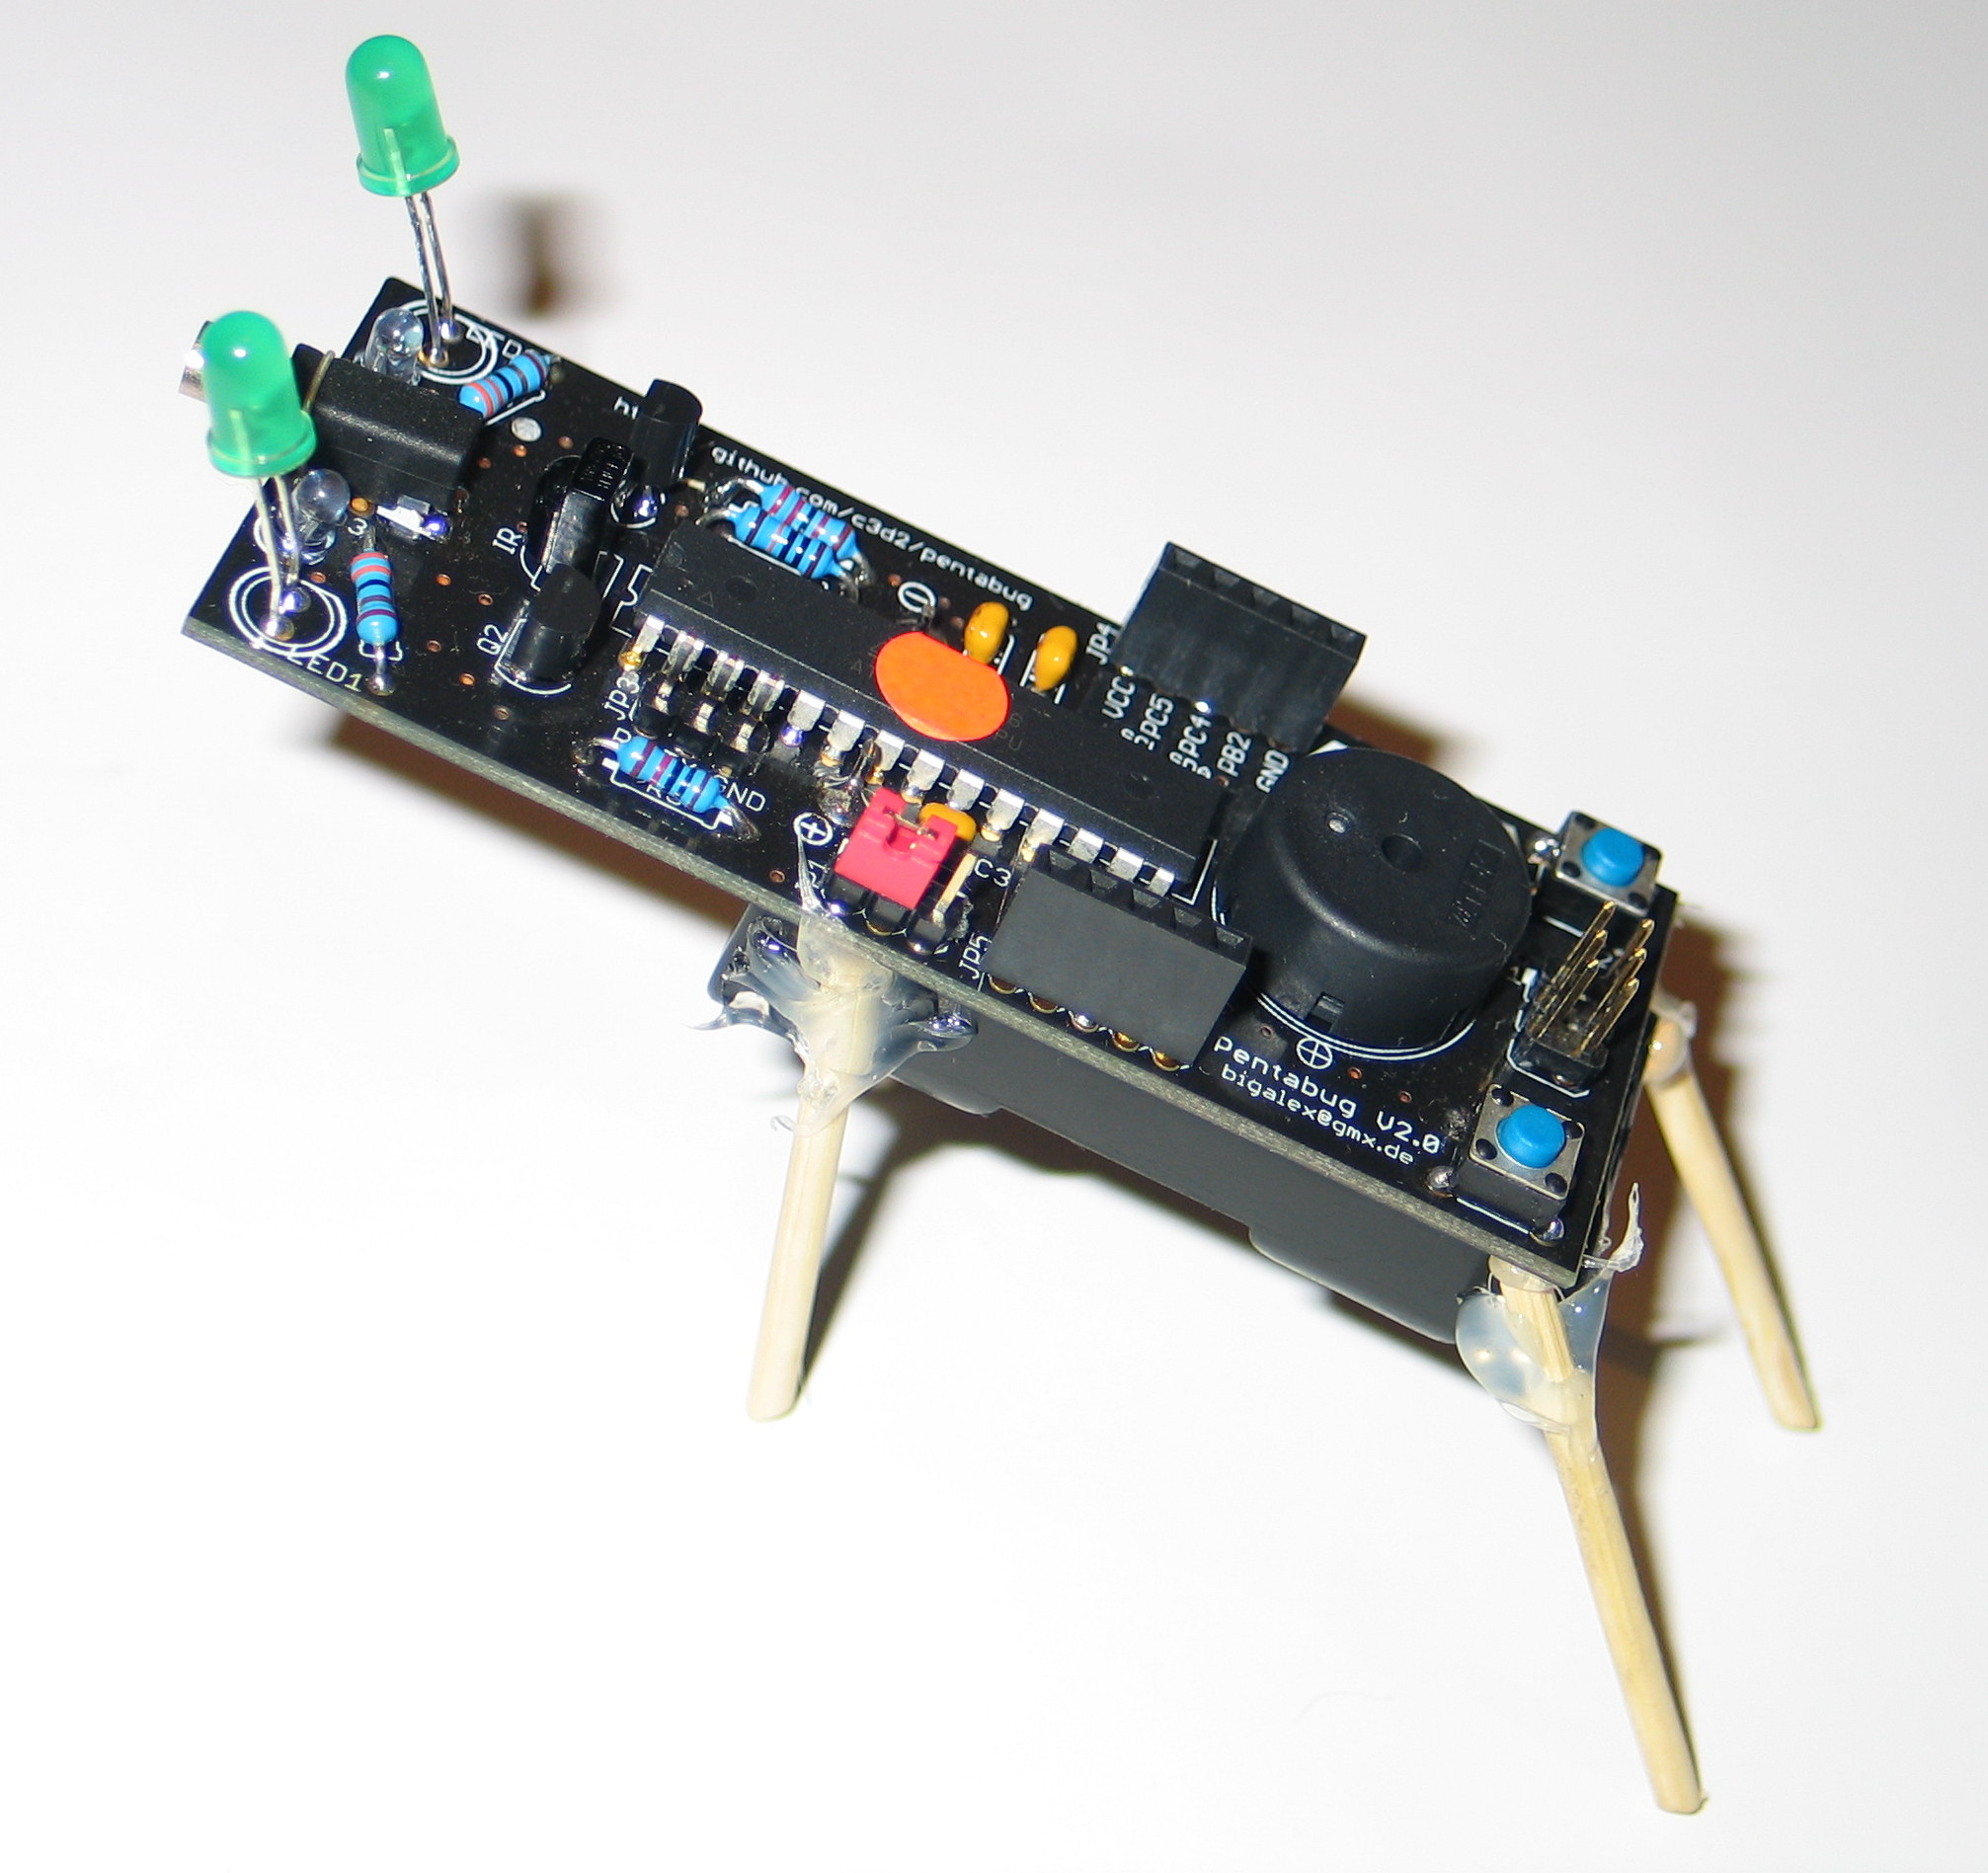
\includegraphics[height=0.5\textheight]{img/pentabug.jpg}
				\end{center}
			}
	\end{itemize}
\end{frame}


\section{Ende}
	\subsection{}
  
\begin{frame}
	\frametitle{Ende}
	\begin{center}
		\textbf{Kontakt: schule@c3d2.de} \\
		\textbf{Fragen?} 
	\end{center}
	\begin{itemize}
		\item<1-> https://c3d2.de
		\item<2-> https://c3d2.de/schule.html
		\item<4-> https://lists.c3d2.de
	\end{itemize}
\end{frame}

\begin{frame}
	\begin{center}
    	
\includegraphics[height=0.5\textheight]{img//cms-text.png}
    \end{center}
\end{frame}

\end{document}
